\date{}
\title{}
\date{}
\begin{document}
\begin{frame}
    \titlepage
\end{frame}

\input{../common/listingsLib}

\begin{frame}{last time}
    \begin{itemize}
    \item user versus kernel mode
    \item system calls
        \begin{itemize}
        \item special instruction
        \item system call wrapper
        \item handler location set at boot
        \end{itemize}
    \item memory protection
    \end{itemize}
\end{frame}

\begin{frame}<1>[label=portalShouldnt]{things programs on portal shouldn't do}
    \begin{itemize}
    \item \myemph<2>{read other user's files}
    \item \myemph<3>{modify OS's memory}
    \item \myemph<3>{read other user's data in memory}
    \item \myemph<4>{hang the entire system}
    \end{itemize}
\end{frame}


\section{memory protection}
\subsubsection{exercise: expected behavior?}
\usetikzlibrary{positioning,shapes.multipart}

\begin{frame}<1-2>[label=memProtectQ]{memory protection}
\begin{itemize}
    \item modifying another program's memory?
\end{itemize}
\lstset{language=myasm,style=small,morekeywords={movq,.word}}
\begin{tabular}{l@{\hspace{.5cm}}|@{\hspace{.5cm}}l}
Program A & Program B \\ \hline
\lstinputlisting{../kernel/memprot-ex1.s} & \lstinputlisting{../kernel/memprot-ex2.s} \\ \hline
~ & ~ \\
\only<2>{result: {\tt \%rax} (in A) is \ldots} 
\only<3->{result: {\tt \%rax} (in A) is {\tt 42}} &
\only<4>{result: {\tt \%rax} (in B) is \ldots} 
\only<5->{result: \myemph{might crash}} \\
\only<3->{(with `normal' multiuser OSes)} \\
\end{tabular}

\begin{visibleenv}<2-5>
\small
A. 42 \hspace{1cm} B. 99 \hspace{1cm} C. 0x10000  \\
D. 42 or 99 (depending on timing/program layout/etc) \\
E. 42 or 99 or program might crash (depending on \ldots) \hspace{1cm} F. something else \\
\end{visibleenv}
\end{frame}

\iftoggle{heldback}{}{\againframe<3>{memProtectQ}}


\subsubsection{preview: shared memory}
\usetikzlibrary{arrows.meta,fit,positioning,shapes.multipart}
\begin{frame}[label=sharedMemAddr]{shared memory}
\begin{tikzpicture}
\tikzset{
    every node/.style={font=\small},
}
\node[align=center] (progAAddr) {Program A \\ addresses};
\node[below=1cm of progAAddr,align=center] (progBAddr) {Program B \\ addresses};
\node[draw, right=1cm of progAAddr,align=center] (translationA) { mapping \\ (set by OS) };
\node[draw, right=1cm of progBAddr,align=center] (translationB) { mapping \\ (set by OS) };
\node[draw,rectangle split, rectangle split parts=6, anchor=north west,label={north:real memory}] (mem) at ([xshift=1cm]translationA.north east) {
    \nodepart{one}
    Program A code 
    \nodepart{two}
    Program B code
    \nodepart{three}
    Program A data
    \nodepart{four}
    Program B data
    \nodepart{five}
    Shared code or data
    \nodepart{six}
    OS data
    \nodepart{seven}
    \ldots
};
\draw[-Latex,green,thick] (progAAddr) -- (translationA) (translationA.east) -- (mem.one west);
\draw[-Latex,green,thick] (translationA.east) -- (mem.three west);
\draw[-Latex,blue,thick] (progBAddr) -- (translationB) (translationB.east) -- (mem.two west);
\draw[-Latex,blue,thick] (translationB.east) -- (mem.four west);
\draw[-Latex,green,ultra thick,dotted] (translationA.east) -- (mem.six west);
\draw[-Latex,blue,ultra thick,dotted] (translationB.east) -- (mem.six west);
    \node[inner sep=0mm,fit=(mem.five split east) (mem.four split west),draw=red,ultra thick] {};
    \begin{pgfonlayer}{bg}
    \node[inner sep=0mm,fit=(mem.five split east) (mem.four split west),draw=red,fill=red!10,ultra thick] {};
    \end{pgfonlayer}
\draw[-Latex,red,ultra thick] (translationA.east) -- (mem.five west);
\draw[-Latex,red,ultra thick] (translationB.east) -- (mem.five west);
\end{tikzpicture}
\end{frame}

\begin{frame}[fragile,label=shmMmap]{one way to set shared memory on Linux}
\lstset{style=smaller,language=C++}
\begin{lstlisting}
/* regular file, OR: */
int fd = open("/tmp/somefile.dat", O_RDWR);
/* special in-memory file */
int fd = shm_open("/name", O_RDWR);
...
/* make file's data accessible as memory */
void *memory = mmap(NULL, size, PROT_READ | PROT_WRITE,
                    MAP_SHARED, fd, 0);
\end{lstlisting}
\begin{itemize}
    \item mmap: ``map'' a file's data into your memory
        \begin{itemize}
        \item if MAP\_SHARED: same data for everyone mapping the file
        \end{itemize}
    \item will discuss a bit more when we talk about virtual memory
    \item part of how Linux loads dynamically linked libraries
\end{itemize}
\end{frame}


% FIXME: talk about ``crash'' in mem protect Q case
\section{extending system calls: exception idea}
\againframe<5>{memProtectQ}
\usetikzlibrary{shapes.geometric}

\begin{frame}{program crashing?}
\begin{itemize}
\item what happens on processor when program crashes?
\vspace{.5cm}
\item other program informed of crash to display message
\item use processor to run some other program
\vspace{.5cm}
\item<2-> how does hardware do this?
\item<2-> would be complicated to tell about other programs, etc.
\item<2-> instead: hardware runs designated OS routine
\end{itemize}
\end{frame}

\begin{frame}{exceptions}
\begin{itemize}
\item recall: system calls --- software asks OS for help
\vspace{.5cm}
\item also cases where hardware asks OS for help
\item different triggers than system calls
\item but \myemph<2>{same mechanism as system calls}:
    \begin{itemize}
    \item switch to kernel mode (if not already)
    \item call OS-designated function
    \end{itemize}
\end{itemize}
\end{frame}

\begin{frame}{exceptions [Venn diagram]}
\begin{tikzpicture}
\node[very thick,draw,ellipse,blue,fill=blue!10,label={south:exceptions},minimum width=15cm,minimum height=6cm] (except) {};
\node[very thick,draw,circle,red,fill=red!10,label={[align=center]center:system\\calls},
      minimum width=3cm] (syscalls) 
    at ([xshift=-3cm,yshift=1cm]except.center){};
\node[very thick,draw,circle,red,fill=red!10,label={[align=center]center:faults\\\small (example:\\\small segfault)},
      minimum width=3cm] (fault) 
    at ([xshift=3cm,yshift=-1cm]except.center){};
\node[very thick,draw,circle,red,fill=red!10,label={[align=center]center:interrupts\\\small (example: I/O)},
      minimum width=3cm] (intr) 
    at ([xshift=0cm,yshift=0cm]except.center){};
\end{tikzpicture}
\end{frame}


\subsection{reasons for exceptions, generally}
\usetikzlibrary{decorations.pathreplacing}

\begin{frame}<0>[label=exceptTypesN]{types of exceptions}
\begin{itemize}
\item \tikzmark{trap bot}\myemph<2>{system calls}
    \begin{itemize}
    \item intentional --- ask OS to do something
    \end{itemize}
\item \tikzmark{fault bot}\myemph<3>{errors/events in programs}
    \begin{itemize}
    \item \myemph<8>{memory not in address space} (``Segmentation fault'')
    \item \myemph<9>{privileged instruction}
    \item \myemph<10>{divide by zero, invalid instruction}
    \item \tikzmark{invalid bot}\ldots
    \end{itemize}
\only<1-4>{(and more we'll talk about later)}
\item<5-> \tikzmark{int bot}\myemph<5>{external --- I/O, etc.}
    \begin{itemize}
    \item \myemph<6>{timer} --- configured by OS to run OS at certain time
    \item \myemph<7>{I/O devices} --- key presses, hard drives, networks, \ldots
    \item \tikzmark{abort bot}hardware is broken (e.g. memory parity error)
    \end{itemize}
\end{itemize}
\begin{tikzpicture}[overlay,remember picture]
    \coordinate (int top) at ([yshift=.6cm]pic cs:int bot);
    \coordinate (fault top) at ([yshift=.6cm]pic cs:fault bot);
    \coordinate (trap top) at ([yshift=.6cm]pic cs:trap bot);
    \coordinate (fault bot) at (pic cs:fault bot);
    \coordinate (over) at ([xshift=-4.5cm]current page.east);
    \coordinate (abort bot)  at (pic cs:abort bot);
    \coordinate (invalid bot)  at ([yshift=.6cm]pic cs:invalid bot);
    \begin{visibleenv}<5->
    \draw[very thick,decorate,decoration={brace}] (int top -| over) -- (abort bot -| over) 
        node[midway,right,font=\large] (async label) {\myemph<5>{asynchronous}};
        \node[anchor=north west,font=\small,align=left] at ([xshift=.15cm,yshift=.3cm]async label.south west) {
            not triggered by \\
            running program
        };
    \end{visibleenv}
    \begin{visibleenv}<4->
    \draw[very thick,decorate,decoration={brace}] (trap top -| over) -- (invalid bot -| over) 
        node[midway,right,font=\large] (sync label) {\myemph<4>{synchronous}};
        \node[anchor=north west,font=\small,align=left] at ([xshift=.15cm,yshift=.3cm]sync label.south west) {
            triggered by \\
            current program
        };
    \end{visibleenv}
\end{tikzpicture}
\end{frame}

\againframe<1-4>{exceptTypesN}

\section{infinite loop}
\againframe<4>{portalShouldnt}

\againframe<5>{exceptTypesN}

\section{exception kinds, summarized}

\begin{frame}{exceptions [Venn diagram]}
\begin{tikzpicture}
\node[very thick,draw,ellipse,blue,fill=blue!10,label={south:exceptions},minimum width=15cm,minimum height=6cm] (except) {};
\node[very thick,draw,circle,red,fill=red!10,label={[align=center]center:system\\calls},
      minimum width=3cm] (syscalls) 
    at ([xshift=-3cm,yshift=1cm]except.center){};
\node[very thick,draw,circle,red,fill=red!10,label={[align=center]center:faults\\\small (example:\\\small segfault)},
      minimum width=3cm] (fault) 
    at ([xshift=3cm,yshift=-1cm]except.center){};
\node[very thick,draw,circle,red,fill=red!10,label={[align=center]center:interrupts\\\small (example: I/O)},
      minimum width=3cm] (intr) 
    at ([xshift=0cm,yshift=0cm]except.center){};
\end{tikzpicture}
\end{frame}


\subsection{exception handling generalized}

\usetikzlibrary{arrows.meta,decorations.pathmorphing}

\begin{frame}{general exception process}
\begin{tikzpicture}
\draw[ultra thick,dashed] (1, -.5) -- (1, -8);
\begin{scope}[every node/.style={anchor=south,align=center}]
    \node at (-4, -.5) {user mode};
    \node at (4, -.5) {kernel mode};
\end{scope}
%\draw[thick,dotted] (-7, -4) -- (7, -4);
\tikzset{
    snake/.style={very thick,decorate,decoration={snake}},
    >=Latex,
    process A/.style={green!70!black},
    process B/.style={red!70!black},
    OS code/.style={blue!70!black},
},
\draw[snake,process A] (-4, -.5) -- (-4, -1.5) coordinate (before enter kernel);
\draw[snake,process A] (6, -2) coordinate (after enter kernel) -- (6, -4) coordinate (before swtch);
\draw[snake,process A] (6, -4) coordinate (after swtch) -- (6, -6) coordinate (before exit kernel);
\draw[snake,process B] (-4, -6.5) coordinate (after exit kernel) -- (-4, -8);
\draw[process A,ultra thick,->,dotted] (before enter kernel) -- (after enter kernel);
\draw[dotted,very thick,<-] (before enter kernel) -- ++(0cm, -.25cm) node[below,align=center,font=\small,fill=white,fill opacity=0.9, inner sep=0.5mm] {
    something triggers exception \\
    maybe the program did \\
    or maybe something else
};
\draw[dotted,very thick,<-] (after enter kernel) -- ++(0cm, .25cm) node[above,align=center,font=\small,fill=white,fill opacity=0.9, inner sep=0.5mm] {
    start exception handler
};
%\draw[ultra thick,->,in=145,out=145] (before swtch) to (after swtch);
\node[align=left,font=\small,fill=white,fill opacity=0.9,anchor=east] at (5.5, -4) {
    OS handles \\ whatever happened
};
\draw[process B,ultra thick,->,dotted] (before exit kernel) -- (after exit kernel);
\draw[dotted,very thick,<-] (after exit kernel) -- ++(0cm, .25cm) node[above,align=center,font=\small,fill=white,fill opacity=0.9, inner sep=0.5mm] {
    go back to running \\
    program code \\
    possibly a different \\
    program than before
};
\draw[dotted,very thick,<-] (before exit kernel) -- ++(0cm, -.25cm) node[below,font=\small,fill=white,fill opacity=0.9, inner sep=0.5mm,align=center] {
    exit exception handler
};
\end{tikzpicture}
\end{frame}


\subsection{operating system runs}
\input{../kernel/contextSwitchIntro}

\subsection{context switches} 
\usetikzlibrary{arrows.meta,calc,positioning,matrix,patterns}


\begin{frame}{OS and time multiplexing}
% FIXME: picture showing zoom of timeline
\begin{itemize}
\item starts running instead of normal program
    \begin{itemize}
    \item mechanism for this: \myemph{exceptions} (later)
    \end{itemize}
\item saves old program counter, registers somewhere
\item sets new registers, jumps to new program counter
\item called \myemph{context switch}
    \begin{itemize}
    \item saved information called \myemph{context}
    \end{itemize}
\end{itemize}
\end{frame}

\begin{frame}<2>[fragile,label=context]{context}
\begin{itemize}
\item all registers values
    \begin{itemize}
        \item \lstinline|%rax| \lstinline|%rbx|, \ldots, \myemph{\tt \%rsp}, \ldots
    \end{itemize}
\item condition codes
\item program counter
\item address space (map from program to real addresses)
\end{itemize}
\end{frame}

\begin{frame}[fragile,label=ctxtSwitchPseudo]{context switch pseudocode}
\lstset{
    style=small,
    language=myasm,
    morekeywords={copy_preexception_pc},
}
\begin{lstlisting}
context_switch(last, next):
  copy_preexception_pc last->pc
  mov rax,last->rax 
  mov rcx, last->rcx 
  mov rdx, last->rdx
  ...
  mov next->rdx, rdx
  mov next->rcx, rcx
  mov next->rax, rax
  jmp next->pc
\end{lstlisting}
\end{frame}

\tikzset{a/.style={fill=blue!30},b/.style={fill=green!30},>=Latex}
\newsavebox{\aContext}
\savebox{\aContext}{
\begin{tikzpicture}
\matrix[tight matrix,nodes={font=\small\tt,a}] (cpuState) {
    \%rax \& SF \\
    \%rbx \& ZF \\
    \%rcx \& PC \\
    \ldots \& \ldots \\
};
\end{tikzpicture}
}
\newsavebox{\bContext}
\savebox{\bContext}{
\begin{tikzpicture}
\matrix[tight matrix,nodes={font=\small\tt,b}] (cpuState) {
    \%rax \& SF \\
    \%rbx \& ZF \\
    \%rcx \& PC \\
    \ldots \& \ldots \\
};
\end{tikzpicture}
}


\begin{frame}{contexts (A running)}
\begin{tikzpicture}
\matrix[tight matrix,label={north:in CPU},nodes={font=\small\tt,a}] (cpuState) {
    \%rax \\
    \%rbx \\
    \%rcx \\
    \%rsp \\
    \ldots \\
    SF \\
    ZF \\
    PC \\
};

\matrix[tight matrix,right=3cm of cpuState, nodes={minimum height=2cm,text width=5cm,align=left},label={in Memory}] (memState) {
    |[a]| {Process A memory: \\ code, stack, etc.} \\
    |[b]| {Process B memory: \\ code, stack, etc.} \\
    |[fill=black!10]|{OS memory: \\ \usebox{\bContext} }\\
};
\draw[thick,dashed,->] (cpuState-4-1.east) -- (memState-1-1.west);
\draw[thick,dashed,->] (cpuState-8-1.east) -- (memState-1-1.west);
\end{tikzpicture}
\end{frame}

\begin{frame}{contexts (B running)}
\begin{tikzpicture}
\tikzset{a/.style={fill=blue!30},b/.style={fill=green!30}}
\matrix[tight matrix,label={north:in CPU},nodes={font=\small\tt,b}] (cpuState) {
    \%rax \\
    \%rbx \\
    \%rcx \\
    \%rsp \\
    \ldots \\
    SF \\
    ZF \\
    PC \\
};
\matrix[tight matrix,right=3cm of cpuState, nodes={minimum height=2cm,text width=5cm},label={north:in Memory}]
    (memState) {
    |[a]| {Process A memory: \\ code, stack, etc.} \\
    |[b]| {Process B memory: \\ code, stack, etc.} \\
    |[fill=black!10]| {OS memory: \\ \usebox{\aContext}} \\
};
\draw[thick,dashed,->] (cpuState-4-1.east) -- (memState-2-1.west);
\draw[thick,dashed,->] (cpuState-8-1.east) -- (memState-2-1.west);
\end{tikzpicture}
\end{frame}




\section{thread idea}
\begin{frame}{threads}
\begin{itemize}
\item thread = illusion of own processor
\vspace{.5cm}
\item own register values
\item own program counter value
\vspace{.5cm}
\item<2-> actual implementation: \\
    many threads sharing one processor
    \begin{itemize}
    \item problem: where are register/program counter values \\
        when thread not active on processor?
    \end{itemize}
\end{itemize}
\end{frame}


\section{not just timers}
\againframe<6>{exceptTypesN}

\subsection{typical I/O pattern}
\begin{frame}{exception patterns with I/O (1)}
    \begin{itemize}
    \item input --- available now:
        \begin{itemize}
        \item exception: device says ``I have input now''
        \item handler: OS stores input for later
        \item exception (syscall): program says ``I want to read input''
        \item handler: OS returns that input
        \end{itemize}
    \item input --- not available now:
        \begin{itemize}
        \item exception (syscall): program says ``I want to read input''
        \item handler: OS runs other things (context switch)
        \item exception: device says ``I have input now''
        \item handler: OS retrieves input
        \item handler: (possibly) OS switches back to program that wanted it
        \end{itemize}
    \end{itemize}
\end{frame}

\begin{frame}{exception patterns with I/O (2)}
    \begin{itemize}
    \item output --- ready now:
        \begin{itemize}
        \item exception (syscall): program says ``I want to output this'
        \item handler: OS sends output to deive
        \end{itemize}
    \item output --- not ready now
        \begin{itemize}
        \item exception (syscall): program says ``I want to output''
        \item handler: OS realizes device can't accept output yet
        \item (other things happen)
        \item exception: device says ``I'm ready for output now''
        \item handler: OS sends output requested earlier
        \end{itemize}
    \end{itemize}
\end{frame}


\input{../kernel/keyInTimeline}

\section{review: exception / context switch}
\begin{frame}{review: definitions}
\begin{itemize}
\item exception: hardware calls OS specified routine
    \begin{itemize}
    \item many possible reasons
    \item system calls: type of exception
    \end{itemize}
\item context switch: OS switches to another thread
    \begin{itemize}
    \item by saving old register values + loading new ones
    \item part of OS routine run by exception
    \end{itemize}
\end{itemize}
\end{frame}


\section{exercise}
\begin{frame}{which of these require exceptions? context switches?}
    \begin{itemize}
    \item A. program calls a function in the standard library
    \item B. program writes a file to disk
    \item C. program A goes to sleep, letting program B run
    \item D. program exits
    \item E. program returns from one function to another function
    \item F. program pops a value from the stack
    \end{itemize}
\end{frame}

\iftoggle{heldback}{}{
\begin{frame}{which require exceptions [answers] (1)}
\begin{itemize}
    \item A. program calls a function in the standard library
        \begin{itemize}
        \item no (same as other functions in program; many standard library functions make no system calls (and do not otherwise trigger exceptions --- for example \texttt{strlen}, \texttt{pow}; also if we consider the calling of a function just the \texttt{call} instruction, then the library functions that do make system calls won't do so until later)
        \end{itemize}
    \item B. program writes a file to disk
        \begin{itemize}
        \item yes (requires kernel mode only operations)
        \end{itemize}
    \item C. program A goes to sleep, letting program B run
        \begin{itemize}
        \item yes (kernel mode usually required to change the address space to acess program B's memory)
        \end{itemize}
\end{itemize}
\end{frame}
\begin{frame}{which require exceptions [answer] (2)}
    \begin{itemize}
    \item D. program exits
        \begin{itemize}
        \item yes (requires switching to another program, which requires accessing OS data + other program's memory)
        \end{itemize}
    \item E. program returns from one function to another function
        \begin{itemize}
        \item no
        \end{itemize}
    \item F. program pops a value from the stack
        \begin{itemize}
        \item no
        \end{itemize}
    \end{itemize}
\end{frame}

\begin{frame}{which require context switches [answer]}
    \begin{itemize}
    \item no: A. program calls a function in the standard library
    \item no: B. program writes a file to disk
        \begin{itemize}
        \item (but might be done if program needs to wait for disk and other things could be run while it does)
        \end{itemize}
    \item yes: C. program A goes to sleep, letting program B run
    \item yes: D. program exits
    \item no: E. program returns from one function to another function
    \item no: F. program pops a value from the stack
    \end{itemize}
\end{frame}
}


\subsection{aside: terms}
\begin{frame}{terms for exceptions}
    \begin{itemize}
    \item terms for exceptions aren't standardized
    \vspace{.5cm}
    \item our readings use one set of terms
    \begin{itemize}
        \item interrupts = externally-triggered
        \item faults = error/event in program
        \item trap = intentionally triggered
        \end{itemize}
    \item all these terms appear differently elsewhere
    \end{itemize}
\end{frame}


\section{process}
\begin{frame}{The Process}
\begin{itemize}
\item \myemph{process} = thread(s) + address space
\item illusion of \myemph{dedicated machine}:
\begin{itemize}
\item thread = illusion of own CPU
\item (process could have multiple threads --- with independent registers)
\item address space = illusion of own memory
\end{itemize}
\end{itemize}
\end{frame}



\section{backup slides}
\begin{frame}{backup slides}
\end{frame}


\subsection{exercise: why not check}
\begin{frame}{keeping permissions?}
    \begin{itemize}
    \item which of the following would still be secure?
    \vspace{.5cm}
    \item A. performing authorization checks in the standard library in addition to system call handlers
    \item B. performing authorization checks in the standard library instead of system call handlers
    \item C. making the user ID a system call argument rather than storing it persistently in the OS's memory
    \end{itemize}
\end{frame}


\subsubsection{address spaces}
\input{../kernel/memProtectAddressSpaces}

\subsection{timing nothing}
\begin{frame}{an infinite loop}
\lstinputlisting[language=C]{../kernel/loop.c}
\begin{itemize}
\item If I run this on a shared department machine, can you still use it? \\
\ldots if the machine only has one core?
\end{itemize}
\end{frame}

\begin{frame}{timing nothing}
\lstinputlisting[firstline=18,language=C]{../kernel/timedloop.c}
\begin{itemize}
\item same instructions --- \myemph{same difference} each time?
\end{itemize}
\end{frame}

\begin{frame}{doing nothing on a busy system}
    % FIXME: wider versions?
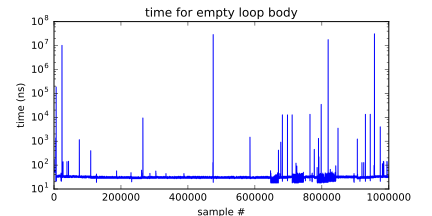
\includegraphics[width=\textwidth]{../kernel/empty-samples}
\end{frame}

\begin{frame}{doing nothing on a busy system}
\includegraphics[width=\textwidth]{../kernel/empty-samples-big-marked}
\end{frame}



\section{time multiplexing}
\usetikzlibrary{arrows.meta,patterns}

\begin{frame}\frametitle{time multiplexing}
\begin{tikzpicture}
\tikzset{
    prog1/.style={draw,fill=cyan!70},
    prog2/.style={draw,fill=green,visible on=<3->},
    prog3/.style={draw,fill=violet!30,visible on=<3->},
    proglabel/.style={font=\tt\scriptsize},
    labelprog1/.style={execute at begin node={\strut loop.exe}},
    labelprog2/.style={execute at begin node={\strut ssh.exe},visible on=<3->},
    labelprog3/.style={execute at begin node={\strut firefox.exe},visible on=<3->},
}
\begin{scope}[xscale=1.5,yscale=1]
\foreach \s/\e/\p [count=\x] in {0/2/1,2/3/2,3/5/3,5/6/1,6/7/2}{
    \draw[prog\p] (\s, 0) rectangle (\e, 1) coordinate[midway] (mid-\x);
    \node[anchor=center,proglabel,labelprog\p] at (mid-\x) {};
}
\end{scope}
\node[anchor=east] at (-0.25, 0.5) {processor:};
% FIXME: system
\begin{scope}[yscale=1,yshift=-2.5mm]
\draw[thick,-Latex] (1,0) node[left] {time} -- (10.5,0);
\end{scope}
\begin{visibleenv}<2->
    \begin{scope}[xscale=1.5]
    \draw[red,thick] (1.9,-.1) coordinate (firstStart) rectangle (2.0, 1.1);
    \draw[red,thick] (5.1,-.1) coordinate (lastEnd) rectangle (5.0, 1.1);
    \end{scope}
    \node[anchor=north west,font=\small\tt,align=left] (asmPre) at (0, -1) {
... \\
loop: ... \\
\hspace{1cm}... \\
\hspace{1cm}jmp loop \\
loop: ... \\
\hspace{1cm}...
    };
    \draw[red, ultra thick] ([xshift=-1cm,yshift=-.2cm]asmPre.south west) -- ([xshift=1cm,yshift=-.2cm]asmPre.south east) node [draw=none,midway,fill=white,
        inner sep=3pt] 
        {million cycle delay};
    \node[anchor=north west,font=\small\tt,align=left] (asmPost) at ([yshift=-.5cm]asmPre.south west) {
\hspace{1cm}... \\
\hspace{1cm}jmp loop \\
loop: ... \\
\hspace{1cm}...
    };
\end{visibleenv}
\end{tikzpicture}
\end{frame}



\subsection{crash timeline}
\input{../kernel/crashTimeline}

\subsection{exception table}


\ifdefined\codeBoxA\else\newsavebox\codeBoxA\fi
\begin{lrbox}{\codeBoxA}
\lstset{
    language=myasm,
    style=script,
}
\begin{lstlisting}
handle_divide_by_zero:
  movq %rax, save_rax
  movq %rbx, save_rbx
  ...
\end{lstlisting}
\end{lrbox}

\ifdefined\codeBoxB\else\newsavebox\codeBoxB\fi
\begin{lrbox}{\codeBoxB}
\lstset{
    language=myasm,
    style=script,
}
\begin{lstlisting}
handle_system_call:
  movq %rax, save_rax
  movq %rbx, save_rbx
  ...
\end{lstlisting}
\end{lrbox}

\ifdefined\codeBoxC\else\newsavebox\codeBoxC\fi
\begin{lrbox}{\codeBoxC}
\lstset{
    language=myasm,
    style=script,
}
\begin{lstlisting}
handle_keyboard_interrupt:
  movq %rax, save_rax
  movq %rbx, save_rbx
  ...
\end{lstlisting}
\end{lrbox}

\begin{frame}[label=locating,fragile]{locating exception handlers (one strategy)}
\begin{tikzpicture}
\tikzset{
    >=Latex,
    every node/.style={font=\small},
}
\matrix[tight matrix,
    nodes={text width=3cm,font=\small},
    column 1/.append style={nodes={draw=none}},
    column 2/.append style={nodes={text width=1.5cm}},
    row 1/.append style={nodes={draw=none}},
    label={[inner sep=0mm,align=center]north:{{\bfseries exception table} (in memory)}},
    label distance=1mm,
] (eTable) {
    |[align=center]| address \& pointer \\
    base + {\tt 0x000} \& ~ \\
    base + {\tt 0x008} \& ~ \\
    base + {\tt 0x010} \& ~ \\
    base + {\tt 0x018} \& ~ \\
    |[align=center]| \ldots \& |[draw=none,align=center]| \ldots \\
    base + {\tt 0x108} \& ~ \\
    |[align=center]| \ldots \& |[draw=none,align=center]| \ldots \\
    base + {\tt 0x400} \&  ~ \\
    |[align=center]| \ldots \& |[draw=none,align=center]| \ldots \\
};
\node[draw,text width=2.8cm, align=center, anchor=south] (baseReg) at ([yshift=1cm,xshift=5mm]eTable-1-1.north west){ exception table base register };
\draw[dashed,very thick,->] ([xshift=-1.2cm]baseReg.south) |- (eTable-2-1.west);
\node[draw,anchor=north west] (hDivZero) at ([xshift=2cm,yshift=2cm]eTable-2-2.north east) {
\usebox{\codeBoxA}
};
\node[draw,anchor=north west] (hSyscall) at ([yshift=-2.5cm]hDivZero.south west){
\usebox{\codeBoxB}
};
\node[draw,anchor=north west] (hKbd) at ([yshift=-.5cm,xshift=2cm]hDivZero.south west){
\usebox{\codeBoxC}
};
\draw[->,thick] (eTable-2-2.center) -- ++(2,0) |- ([yshift=-1ex]hDivZero.north west);
\draw[thick] (eTable-3-2.center) -- ++ (1, 0) node[right]{\ldots};
\draw[thick] (eTable-4-2.center) -- ++ (1, 0) node[right]{\ldots};
\draw[thick] (eTable-5-2.center) -- ++ (1, 0) node[right]{\ldots};
\draw[->,thick] (eTable-7-2.center) -- ++(2,0) |- ([yshift=-1ex]hKbd.north west);
\draw[->,thick] (eTable-9-2.center) -- ++(2,0) |- ([yshift=-1ex]hSyscall.north west);
\end{tikzpicture}
\end{frame}



\subsection{key-in timeline}
\input{../kernel/keyInTimeline}

\subsection{nested exceptions?}
\usetikzlibrary{fit,positioning,shapes.misc}

\ifdefined\codeBoxA\else\newsavebox\codeBoxA\fi
\begin{lrbox}{\codeBoxA}
\lstset{
    language=myasm,
    style=small,
    moredelim=**[is][\btHL<1>]{@1}{@},
    moredelim=**[is][\btHL<2>]{@2}{@},
    moredelim=**[is][\btHL<3>]{@3}{@},
    moredelim=**[is][\btHL<4>]{@4}{@},
}
\begin{lstlisting}
handle_timer_interrupt:
  save_old_pc @2save_pc@
  movq %r15, @2save_r15@
  /* key press here */
\end{lstlisting}
\end{lrbox}
\ifdefined\codeBoxB\else\newsavebox\codeBoxB\fi
\begin{lrbox}{\codeBoxB}
\lstset{
    language=myasm,
    style=small,
}
\begin{lstlisting}
  movq %r14, save_r14
  ...
\end{lstlisting}
\end{lrbox}
\ifdefined\codeBoxC\else\newsavebox\codeBoxC\fi
\begin{lrbox}{\codeBoxC}
\lstset{
    language=myasm,
    style=small,
}
\begin{lstlisting}
handle_keyboard_interrupt:
  save_old_pc save_pc
  movq %r15, save_r15
  movq %r14, save_r14
  movq %r13, save_r13
  ...
\end{lstlisting}
\end{lrbox}

\begin{frame}[fragile,label=nestedExcept]{exceptions in exceptions}
\begin{tikzpicture}
\node (code1) {
\usebox{\codeBoxA}
};
\node[anchor=north west] (code1b) at ([yshift=1mm]code1.south west) {
\usebox{\codeBoxB}
};
\begin{visibleenv}<2->
\node[draw,thick,blue!70!black,anchor=north west] (code2) at ([yshift=0.5cm,xshift=5cm]code1b.south west) {
\usebox{\codeBoxC}
};
\draw[very thick,blue,-Latex] (code1.south west) -- (code1.south east) -- (code1.south east |- code2.north);
\end{visibleenv}
\begin{visibleenv}<3->
\node[draw,red,ultra thick,cross out,fit=(code2)] at (code2) {};
\node[left=.1cm of code2,red] {
    oops, overwrote saved values?
};
\end{visibleenv}
\end{tikzpicture}
\end{frame}

\begin{frame}{interrupt disabling}
\begin{itemize}
\item CPU supports \myemph{disabling} (most) interrupts
\item interrupts will \myemph{wait} until it is reenabled
\item CPU has extra state:
    \begin{itemize}
    \item are interrupts enabled?
    \item is keyboard interrupt pending?
    \item is timer interrupt pending?
    \end{itemize}
\end{itemize}
% FIXME: shwoing logic?
\end{frame}

\ifdefined\codeBoxA\else\newsavebox\codeBoxA\fi
\begin{lrbox}{\codeBoxA}
\lstset{
    language=myasm,
    style=small,
    moredelim=**[is][\btHL<1|handout:1>]{@1}{@},
    moredelim=**[is][\btHL<2|handout:2>]{@2}{@},
    moredelim=**[is][\btHL<3|handout:3>]{@3}{@},
    moredelim=**[is][\btHL<4|handout:4>]{@4}{@},
}
\begin{lstlisting}
handle_timer_interrupt:
  /* interrupts automatically disabled here */
  movq %rsp, save_rsp
  save_old_pc save_pc
  /* key press here */
  jmpIfFromKernelMode skip_exception_stack
  movq current_exception_stack, %rsp
skip_set_kernel_stack:
  pushq save_rsp
  pushq save_pc
  enable_intterupts
  pushq %r15
  ...
\end{lstlisting}
\end{lrbox}

\ifdefined\codeBoxB\else\newsavebox\codeBoxB\fi
\begin{lrbox}{\codeBoxB}
\lstset{
    language=myasm,
    style=small,
    moredelim=**[is][\btHL<1|handout:1>]{@1}{@},
    moredelim=**[is][\btHL<2|handout:2>]{@2}{@},
    moredelim=**[is][\btHL<3|handout:3>]{@3}{@},
    moredelim=**[is][\btHL<4|handout:4>]{@4}{@},
}
\begin{lstlisting}
  /* interrupt happens here! */
  ...
\end{lstlisting}
\end{lrbox}

\ifdefined\codeBoxC\else\newsavebox\codeBoxC\fi
\begin{lrbox}{\codeBoxC}
\begin{lstlisting}
handle_keyboard_interrupt:
  movq %rsp, save_rsp
  save_old_pc save_pc
  jmpIfFromKernelMode skip_exception_stack
  movq current_exception_stack, %rsp
skip_exception_stack:
  pushq save_rsp
  pushq save_pc
  enable_intterupts
  pushq %r15
  ...
\end{lstlisting}
\end{lrbox}


\begin{frame}[fragile,label=nestedExcept2]{exceptions in exceptions}
\lstset{
    language=myasm,
    style=small,
    moredelim=**[is][\btHL<1|handout:1>]{@1}{@},
    moredelim=**[is][\btHL<2|handout:2>]{@2}{@},
    moredelim=**[is][\btHL<3|handout:3>]{@3}{@},
    moredelim=**[is][\btHL<4|handout:4>]{@4}{@},
}
\begin{tikzpicture}
\node (code1) {
\usebox{\codeBoxA}
};
\node[anchor=north west] (code1b) at ([yshift=1mm]code1.south west) {
\usebox{\codeBoxB}
};
\begin{visibleenv}<3->
\node[draw,thick,blue!70!black,anchor=north west] (code2) at ([yshift=0.5cm,xshift=5cm]code1b.south west) {
\usebox{\codeBoxC}
};
\draw[very thick,blue,-Latex] (code1.south west) -- ([xshift=-2cm]code1.south east) -- ([xshift=-2cm]code1.south east |- code2.north);
\end{visibleenv}

\end{tikzpicture}
\end{frame}

\begin{frame}[fragile,label=disableInt]{disabling interrupts}
\begin{itemize}
\item automatically disabled when exception handler starts
\item also can be done with privileged instruction:
\end{itemize}
\begin{lstlisting}
change_keyboard_parameters:
  disable_interrupts
  ...
  /* change things used by
     handle_keyboard_interrupt here */
  ...
  enable_interrupts
\end{lstlisting}
\end{frame}




\section{exception table + dispatch}
\begin{frame}{exception implementation}
\begin{itemize}
\item detect condition (program error or external event)
\item save current value of PC somewhere
\item jump to \myemph{exception handler} (part of OS)
    \begin{itemize}
    \item jump done without program instruction to do so
    \end{itemize}
\end{itemize}
\end{frame}

\begin{frame}{exception implementation: notes}
\begin{itemize}
\item I describe a \myemph{simplified} version
\item real x86/x86-64 is a bit more complicated
    \begin{itemize}
    \item (mostly for historical reasons)
    \end{itemize}
\end{itemize}
\end{frame}



\subsection{in the context}

\begin{frame}<2>[fragile,label=context]{context}
\begin{itemize}
\item all registers values
    \begin{itemize}
        \item \lstinline|%rax| \lstinline|%rbx|, \ldots, \myemph{\tt \%rsp}, \ldots
    \end{itemize}
\item condition codes
\item program counter
\item address space (map from program to real addresses)
\end{itemize}
\end{frame}



\subsection{context switch pseudocode}

\begin{frame}[fragile,label=ctxtSwitchPseudo]{context switch pseudocode}
\lstset{
    style=small,
    language=myasm,
    morekeywords={copy_preexception_pc},
}
\begin{lstlisting}
context_switch(last, next):
  copy_preexception_pc last->pc
  mov rax,last->rax 
  mov rcx, last->rcx 
  mov rdx, last->rdx
  ...
  mov next->rdx, rdx
  mov next->rcx, rcx
  mov next->rax, rax
  jmp next->pc
\end{lstlisting}
\end{frame}


\subsection{Unix design [full]}
\input{../kernel/unix-design}

\section{exception dispatch}
\begin{frame}{exception implementation}
\begin{itemize}
\item detect condition (program error or external event)
\item save current value of PC somewhere
\item jump to \myemph{exception handler} (part of OS)
    \begin{itemize}
    \item jump done without program instruction to do so
    \end{itemize}
\end{itemize}
\end{frame}

\begin{frame}{exception implementation: notes}
\begin{itemize}
\item I describe a \myemph{simplified} version
\item real x86/x86-64 is a bit more complicated
    \begin{itemize}
    \item (mostly for historical reasons)
    \end{itemize}
\end{itemize}
\end{frame}



\begin{frame}[fragile,label=exceptHandlerRun]{running the exception handler}
\begin{itemize}
    \item hardware saves the \myemph{old program counter} (and maybe more)
    \item identifies location of exception handler via table
    \item then jumps to that location
    \vspace{.5cm}
    \item OS code can save anything else it wants to , etc.
\end{itemize}
\end{frame}





\end{document}
